 \documentclass{beamer}
\title{Scifi-sound}
\author{Charly Ahrendts}
\date{GYPT 2019}
\usetheme{focus}
\usepackage{wrapfig}
\usepackage{tabularx}



\begin{document}
\frame{\titlepage}

\begin{frame}{Task}
Tapping a helical spring can make a sound like a “laser shot” in a science-fiction movie.
Investigate and explain this phenomenon.
\end{frame}
   
%\begin{frame}{Table of Contents}
%  \tableofcontents
%\end{frame}

\section {Basic explanation}
	\begin{frame}{Dispersion}
  \begin{columns}
      \column{\dimexpr.65\textwidth}
			\begin{itemize}
			\item
				Phase velocity of a wave as a function of frequency
			\item
				Frequencies propagate at different velocities through the medium
			\item
				Only in certain materials (solids and liquids)
			\item
				Applies to optical as well as acoustic waves
			\item
				More dense materials are usually more dispersive 
			\end{itemize}
      
      \column{\dimexpr.35\textwidth}
     	 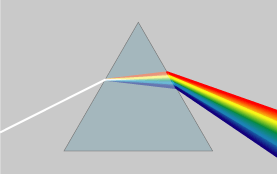
\includegraphics [scale=0.4]{images/prism.png}

    \end{columns}
	
   			
	\end{frame}

	\begin{frame} {Slinky}
	\begin{columns}
      \column{\dimexpr.65\textwidth}
		\begin{itemize}
			\item
			Helical spring often made of metal
			\item
			Highly dispersive
			\item
			Tapping it produces a short signal consisting of multiple frequencies
			\item
			Wave dissects into its component frequencies 
			\item
			Higher frequencies are heard before the lower ones, thus producing the "scifi-sound"
			\end{itemize}
		\column{\dimexpr.35\textwidth}
			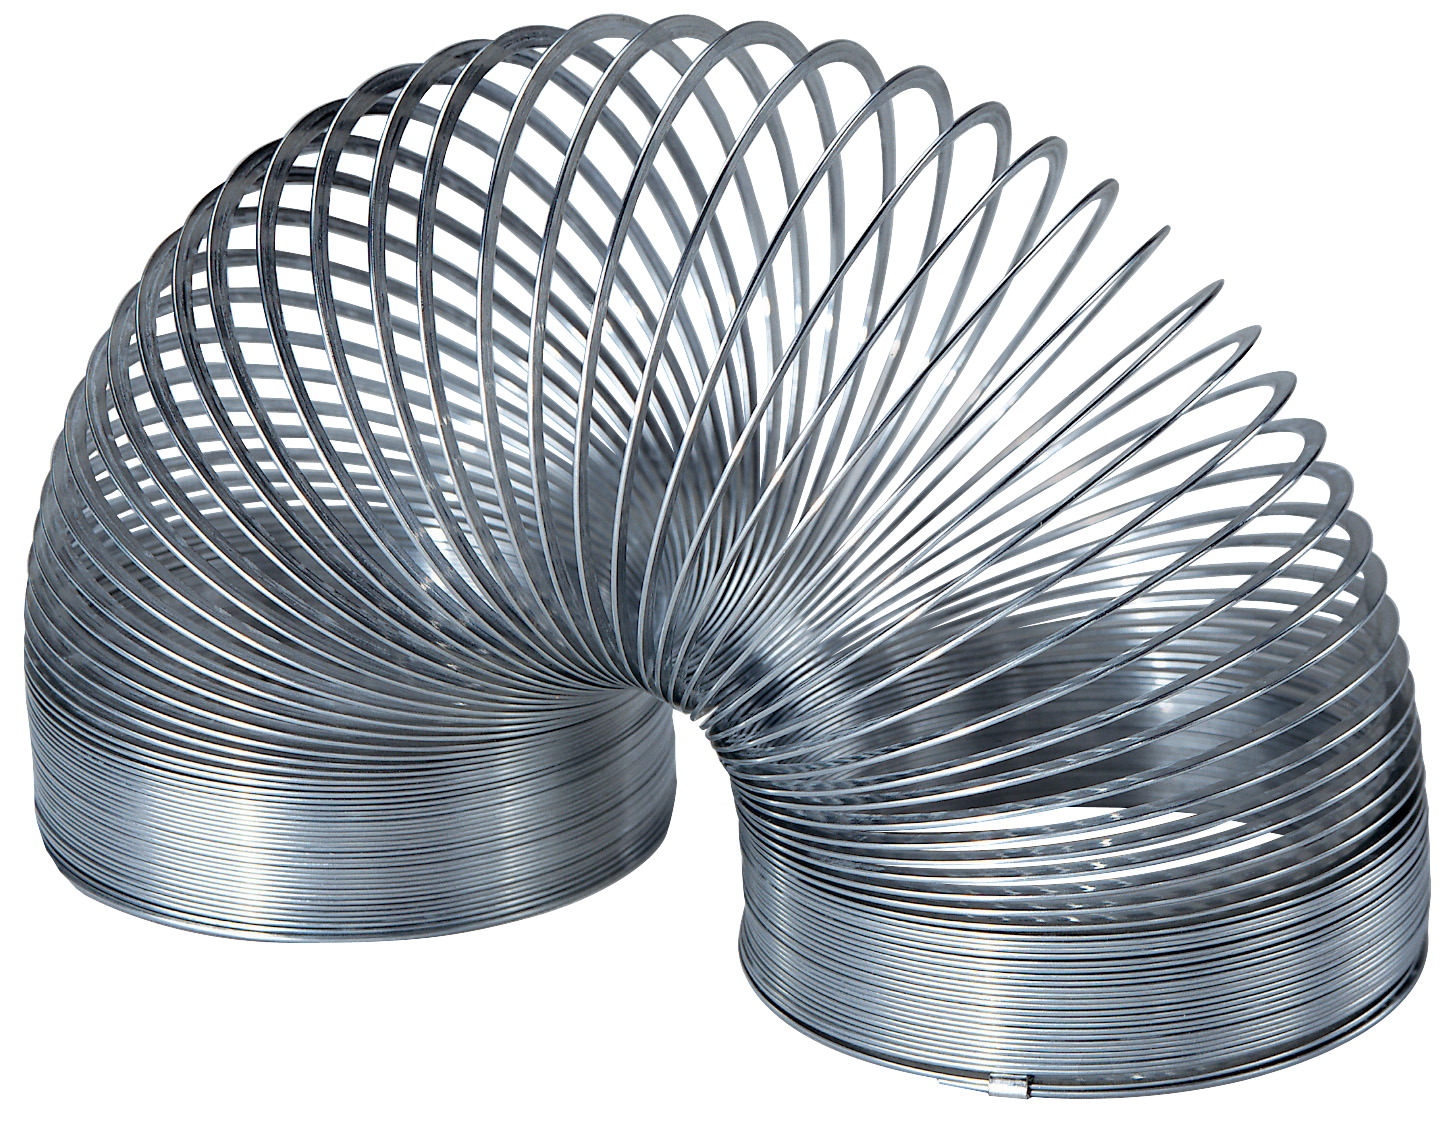
\includegraphics [scale=0.08]{images/slinky.jpg}
			
		\end{columns}
	\end{frame}
	
\section {Experimental setup}
	\begin{frame}{Experimental setup}
	\begin{center}
		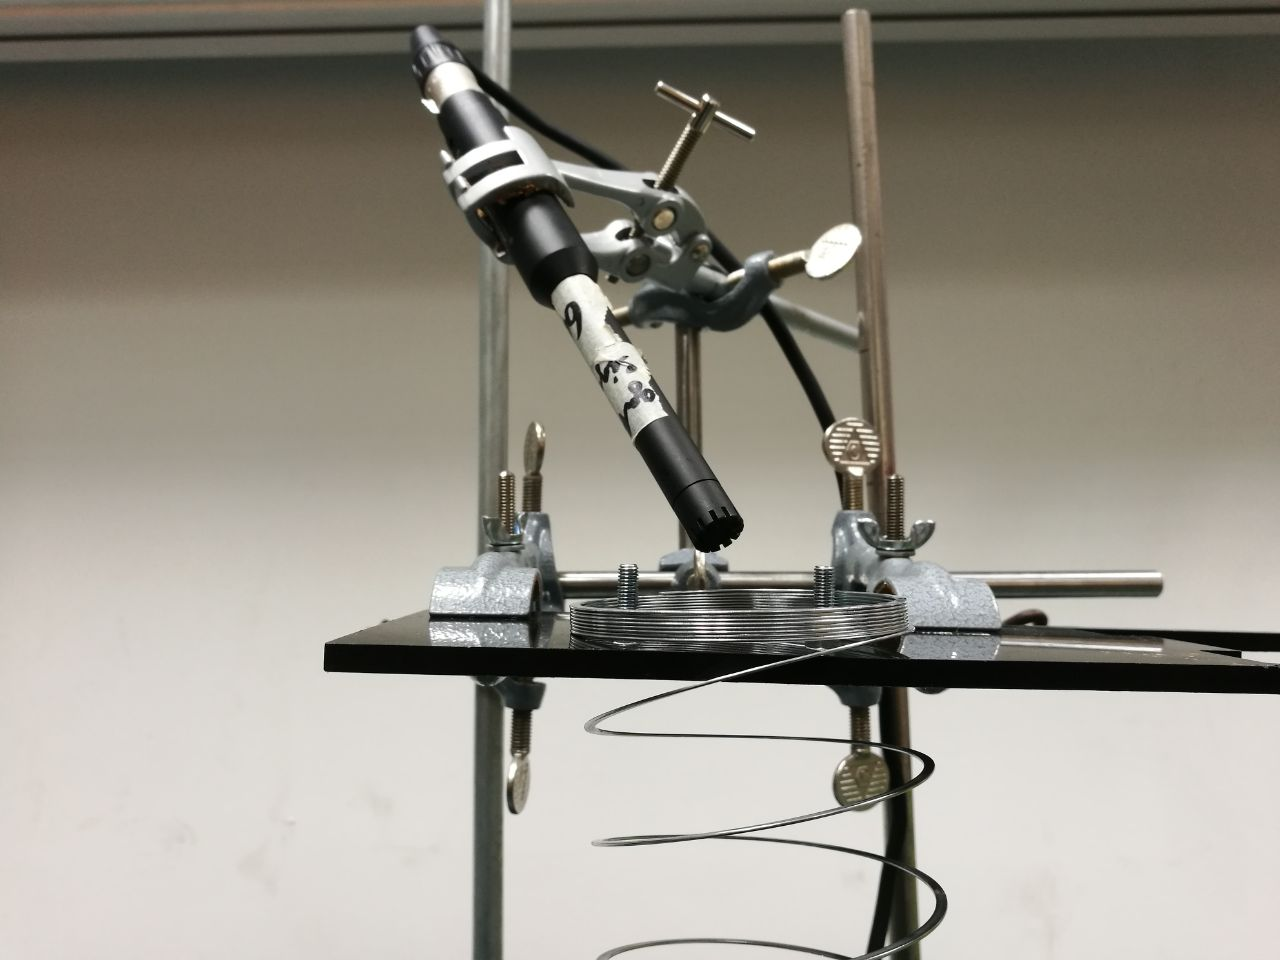
\includegraphics [scale=0.22]{images/better_setup_1.jpg}
		%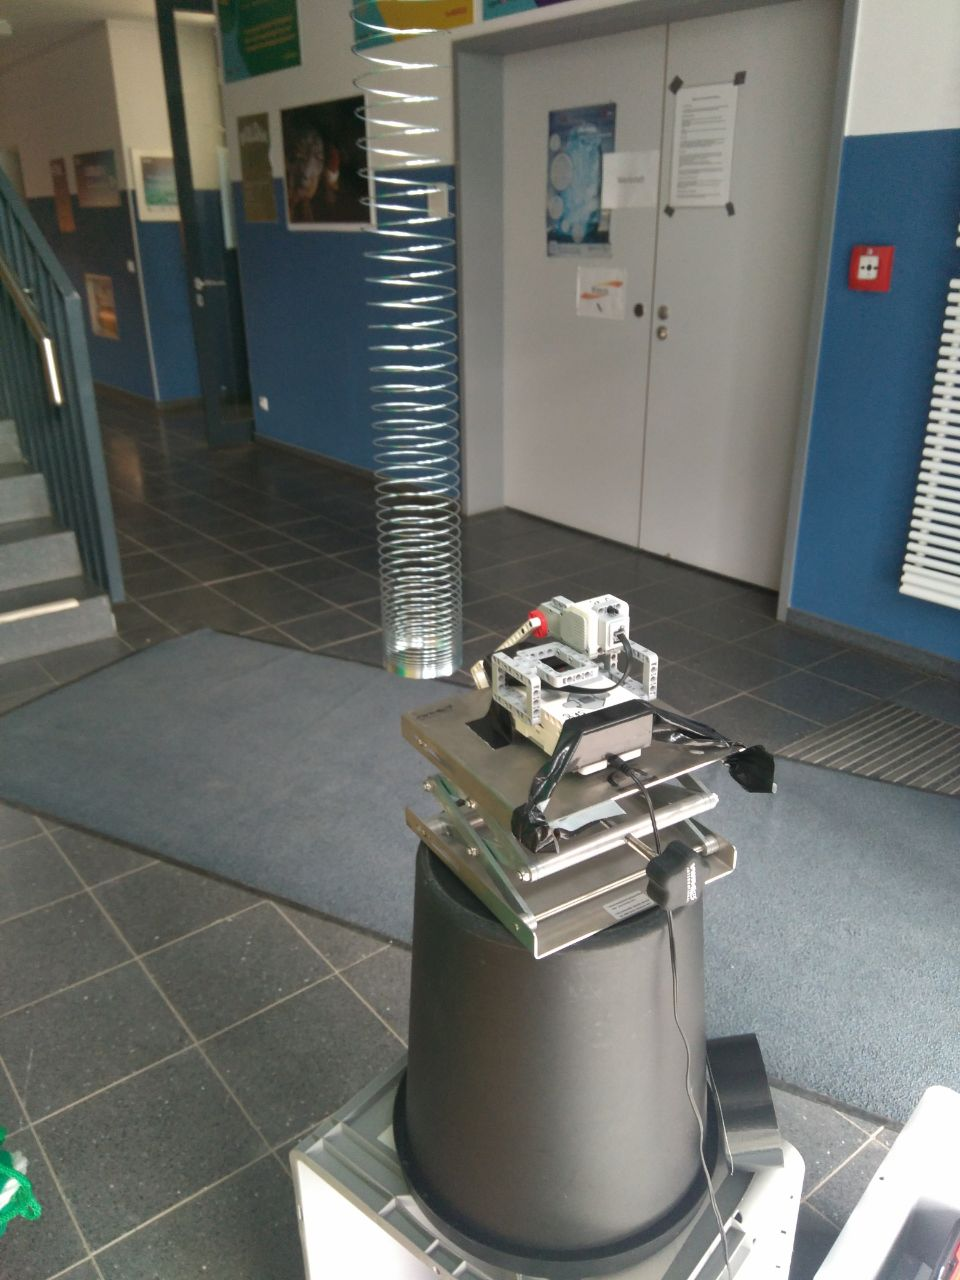
\includegraphics [scale=0.13]{images/setup_1.jpg}
	\end{center}
	\end{frame}


\section {Experimental results}
	\begin{frame}{Response curve metal}
		\begin{center}
		
		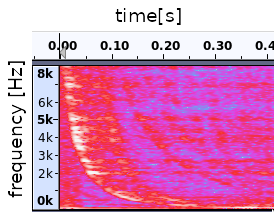
\includegraphics [scale=0.7]{images/echo_1_axies.png}
		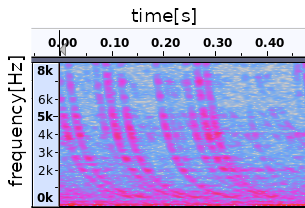
\includegraphics [scale=0.7]{images/echo_2_axies.png}
		\end{center}
	\end{frame}
	
	\begin{frame}{Response curve plastic}
		\begin{center}
			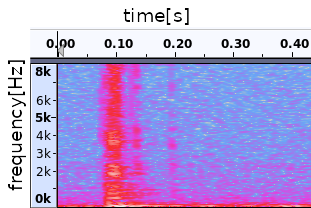
\includegraphics [scale=0.68]{images/plastic.png}
			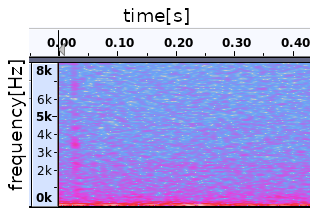
\includegraphics [scale=0.68]{images/plastic_echo.png}
		\end{center}
	\end{frame}

\section {Theory}
	\begin{frame}{Formulas}
		
		Euler-Bernoulli ideal bar equation\footnote{ \tiny{ Parker, Julian, et al. 'Modeling methods for the highly dispersive slinky spring: a
novel musical toy.' Proceedings of the 13th International Conference on Digital
Audio Effects 2010.}}:
		%\begin{equation}
			%\frac{\partial ^2 u }{\partial t^2} = -\kappa ^2 \cdot  \frac{\partial^4 u}  {\partial x^4}  
		%\end{equation}
		
		
		\begin{equation}
			t_D = \frac{1}{2 \sqrt{\pi  \kappa  f}}
		\end{equation}
		
		\begin{equation}
			f(t) = \frac{1} {8 \pi \kappa t^2}
		\end{equation}
		where: \\
		$f =$ frequency [Hz] \\
		$t =$ time [s] \\
		$t_D =$ duration time [s] \\
		$\kappa =$ fit parameter
				
	\end{frame}

	\begin{frame}{Fit parameter $\kappa$}
	$\kappa$ determines how widely spread the frequencies are.\\ It is dependent on material properties, such as:
		\begin{itemize}
		\item
		Density
		\item
		E-Modulus
		%\item
		%Poisson's ratio
		\item
		Length			
		\end{itemize}
	\end{frame}


\section {Theory-Experiment Comparison}
	\begin{frame}{Data processing}
	\begin{center}
	
		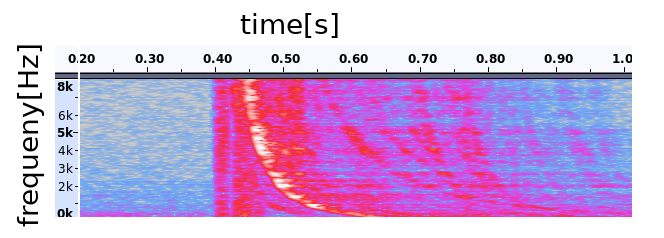
\includegraphics [scale=0.47]{images/axies.png}
		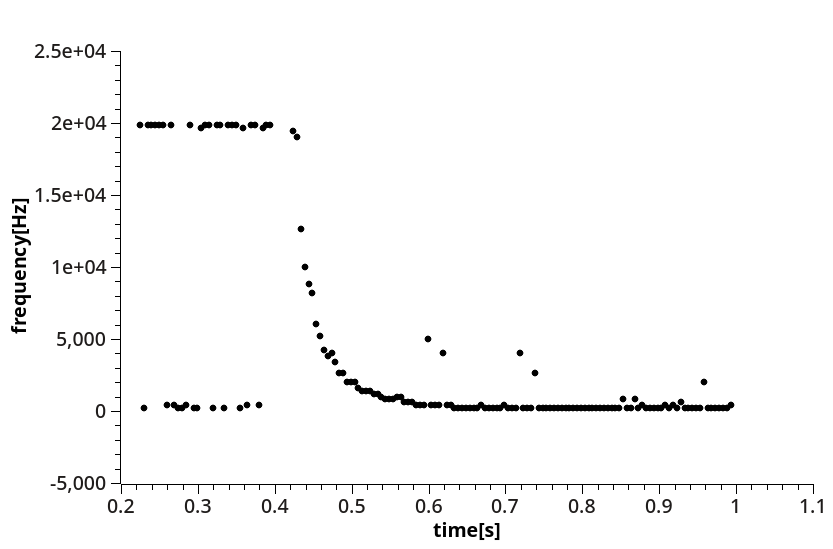
\includegraphics [scale=0.25]{images/converted_csv.png}
	\end{center}

	\end{frame}

	\begin{frame}{Fitted function}
		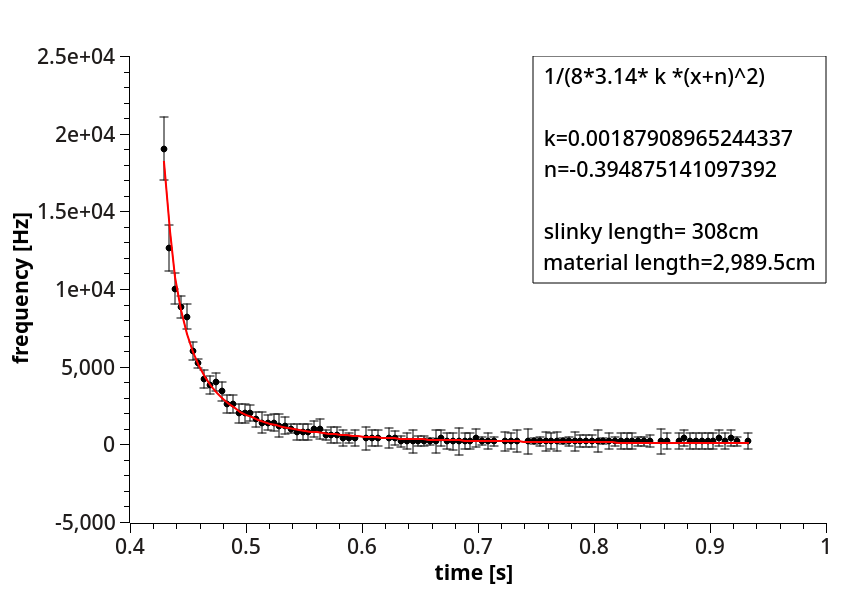
\includegraphics [scale=0.38]{images/legend_and_errors.png}
		
	\end{frame}
	
	\begin{frame}{Direct comparison}
		\begin{center}
			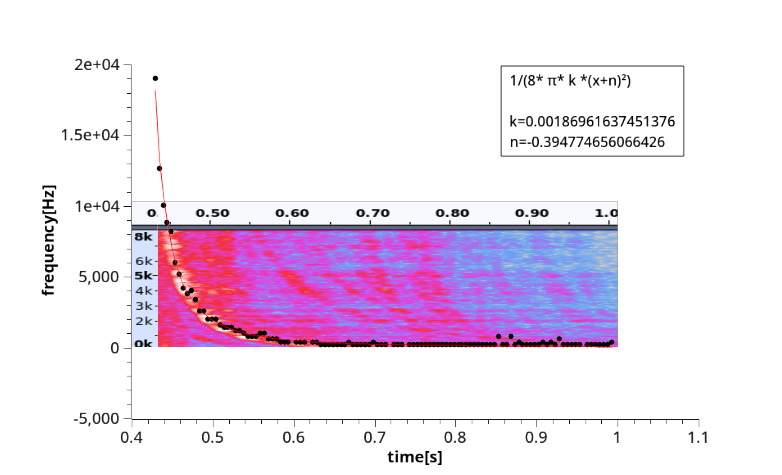
\includegraphics [scale=0.58]{images/comparison.png}
		\end{center}		
	\end{frame}

\section {Conclusion}
	\begin{frame}{Conclusion}
		I was able to:
		\begin{itemize}
		\item
		Explain and reproduce the phenomenon
		\item
		Qualitatively investigate it in a controlled experiment
		\item
		Find a fitting theory 
		\item
		Compare the theory with my measured data
		\end{itemize}
	\end{frame}

	\begin{frame}{Outlook}
	For the future, I plan to:
	\begin{itemize}
	\item
	Further investigate material and length of the spring
	\item
	Investigate the phenomenon in a steel cable
	\item
	Quantify my results
	\item
	$\kappa(length)$ plot
	\end{itemize}
	
	\end{frame}	



\end{document}

